% Options for packages loaded elsewhere
\PassOptionsToPackage{unicode}{hyperref}
\PassOptionsToPackage{hyphens}{url}
\documentclass[
]{article}
\usepackage{xcolor}
\usepackage{amsmath,amssymb}
\setcounter{secnumdepth}{-\maxdimen} % remove section numbering
\usepackage{iftex}
\ifPDFTeX
  \usepackage[T1]{fontenc}
  \usepackage[utf8]{inputenc}
  \usepackage{textcomp} % provide euro and other symbols
\else % if luatex or xetex
  \usepackage{unicode-math} % this also loads fontspec
  \defaultfontfeatures{Scale=MatchLowercase}
  \defaultfontfeatures[\rmfamily]{Ligatures=TeX,Scale=1}
\fi
\usepackage{lmodern}
\ifPDFTeX\else
  % xetex/luatex font selection
\fi
% Use upquote if available, for straight quotes in verbatim environments
\IfFileExists{upquote.sty}{\usepackage{upquote}}{}
\IfFileExists{microtype.sty}{% use microtype if available
  \usepackage[]{microtype}
  \UseMicrotypeSet[protrusion]{basicmath} % disable protrusion for tt fonts
}{}
\makeatletter
\@ifundefined{KOMAClassName}{% if non-KOMA class
  \IfFileExists{parskip.sty}{%
    \usepackage{parskip}
  }{% else
    \setlength{\parindent}{0pt}
    \setlength{\parskip}{6pt plus 2pt minus 1pt}}
}{% if KOMA class
  \KOMAoptions{parskip=half}}
\makeatother
\usepackage{graphicx}
\makeatletter
\newsavebox\pandoc@box
\newcommand*\pandocbounded[1]{% scales image to fit in text height/width
  \sbox\pandoc@box{#1}%
  \Gscale@div\@tempa{\textheight}{\dimexpr\ht\pandoc@box+\dp\pandoc@box\relax}%
  \Gscale@div\@tempb{\linewidth}{\wd\pandoc@box}%
  \ifdim\@tempb\p@<\@tempa\p@\let\@tempa\@tempb\fi% select the smaller of both
  \ifdim\@tempa\p@<\p@\scalebox{\@tempa}{\usebox\pandoc@box}%
  \else\usebox{\pandoc@box}%
  \fi%
}
% Set default figure placement to htbp
\def\fps@figure{htbp}
\makeatother
\setlength{\emergencystretch}{3em} % prevent overfull lines
\providecommand{\tightlist}{%
  \setlength{\itemsep}{0pt}\setlength{\parskip}{0pt}}
\usepackage{bookmark}
\IfFileExists{xurl.sty}{\usepackage{xurl}}{} % add URL line breaks if available
\urlstyle{same}
\hypersetup{
  hidelinks,
  pdfcreator={LaTeX via pandoc}}

\author{}
\date{}

\begin{document}

\section{Interference of Two Particle-like States with a Spread Phase:
Feature Points of Relative Configuration and a Structural Correspondence
with Statistics (Observational Note,
Draft)}\label{interference-of-two-particle-like-states-with-a-spread-phase-feature-points-of-relative-configuration-and-a-structural-correspondence-with-statistics-observational-note-draft}

\textbf{Author}: Noriaki Kihara \textbf{Affiliation}: WF System Co.,
Ltd.~/ Faculty of Engineering Science, Osaka University (graduate)
\textbf{ORCID}:
\href{https://orcid.org/0009-0004-6753-4020}{0009-0004-6753-4020}
\textbf{Version}: v1.0 (publication candidate, not peer-reviewed)
\textbf{Date}: June 2026 \textbf{License}: CC BY 4.0 \textbf{Concept
DOI}:
\href{https://doi.org/10.5281/zenodo.20544004}{10.5281/zenodo.20544004}
\textbf{Version DOI (v1.0)}:
\href{https://doi.org/10.5281/zenodo.20544005}{10.5281/zenodo.20544005}

\begin{center}\rule{0.5\linewidth}{0.5pt}\end{center}

\subsection{Character of this note}\label{character-of-this-note}

\textbf{This is an observational note in the form of a thought
experiment. It is not a proof paper or a claim paper.}

This note is a sequel to the preceding note {[}1{]} (Central projection
of a vacuum universe and particle-like states with a spread phase). The
preceding note defined a single particle-like state as a phase-bearing
local mode with a spread phase on the subjective geometry
\(S^4(R_{\mathrm U})\), going as far as setting its spread to
\(W_a=2R_a\) (a model convention), and explicitly deferred the relative
phase, interference, and statistics of multiple particles to a
subsequent note. The present note treats the minimal case of that
deferred part---\textbf{two particle-like states with the same spread
phase}---on a closed one-dimensional relational setting.

What distinguishes this note from the preceding one is that most of its
conclusions are obtained as \textbf{closed elementary Fourier-series
computations}. That is, we obtain in closed form the spectrum and the
total squared norm of the superposition of two particles represented as
rectangular standing waves, and from these we observe the discrete
feature points appearing within the continuous relative position
(fusion, orthogonality, complete cancellation) and the admissibility of
overlap depending on symmetrization / antisymmetrization (a structural
correspondence with the exchange symmetry of quantum statistics).

This note does not modify standard quantum theory, general relativity,
or special relativity. It proposes no new physical theory, proves no new
mathematical theorem, and changes no observable prediction. What it does
is to re-arrange and observe, from the single viewpoint of the relative
configuration of two particles, known structures---the Fourier series of
a square wave and Parseval's relation {[}4{]}, the exchange symmetry of
quantum statistics (Bose/Fermi), and the spread phase {[}1{]} and
central projection {[}2,3{]} of the preceding notes.

This note does not assert any of the following:

\begin{itemize}
\tightlist
\item
  any change to the mathematical predictions of the Standard Model,
  quantum theory, or relativity;
\item
  identification of a particle-like state with a concrete particle such
  as an electron, photon, or quark;
\item
  derivation of the spin-statistics theorem, the Hilbert-space
  structure, or quantum field theory;
\item
  any new observable prediction, or proof of any new mathematical
  theorem;
\item
  that the interference structure of this note ``derives'' actual
  quantum statistics (we remain at the level of observing a structural
  correspondence).
\end{itemize}

Evaluation and interpretation are left to the reader.

\begin{center}\rule{0.5\linewidth}{0.5pt}\end{center}

\subsection{Abstract}\label{abstract}

In the preceding note {[}1{]}, a particle-like state was defined as a
phase-bearing local mode with a spread phase on the subjective geometry,
with spread \(W_a=2R_a=2/\nu_{R,a}\) (a model convention). Here we
superpose two particle-like states with the same frequency \(\nu\) on a
closed one-dimensional relational setting and observe their
interference. Representing each particle as a rectangular standing wave
consisting of odd harmonics, the amplitude of the \(n\)-th harmonic of
the superposition, in terms of the relative position \(f\) measured in
fundamental wavelengths, is \(A_n=\tfrac{2}{n}\cos(n\pi f)\), and the
total squared norm (an energy-like quantity) is the triangle wave
\(E(f)=\tfrac{\pi^2}{4}(1-2f)\) (\(0\le f\le\tfrac12\); the
autocorrelation of a square wave). From this we observe that within the
continuous relative position \(f\) there appear discrete feature points
corresponding to fusion (\(f=0\)), orthogonality / independent
coexistence (\(f=\tfrac14\)), and complete cancellation
(\(f=\tfrac12\)). Furthermore, depending on whether the superposition is
symmetrized or antisymmetrized, complete overlap (\(f=0\)) is admissible
(boson-like) or makes the composite field vanish, i.e.~exclusive
(fermion-like). Finally, for unequal frequencies, the strength of
interference is governed by whether odd harmonics are shared
(commensurability); without sharing, interference vanishes and the
placement becomes free. All of this is presented as observations of
structural correspondence; no derivation of quantum statistics is
claimed.

\begin{center}\rule{0.5\linewidth}{0.5pt}\end{center}

\subsection{§1 Starting point---connection to the preceding
note}\label{starting-pointconnection-to-the-preceding-note}

The preceding note {[}1{]} observed that a particle-like state with a
spread phase, \(P_a=(\boldsymbol{\nu}_a,R_a)\), can be placed on the
subjective geometry \(S^4(R_{\mathrm U})\) produced by the central
projection of an exterior-free vacuum universe. There, on the two
grounds that

\begin{itemize}
\tightlist
\item
  position is relational, and no absolute position phase is defined for
  a single particle, and
\item
  on the curved subjective geometry a simple difference of phases is not
  coordinate-invariant,
\end{itemize}

the formulation of the relative phase, interference, and statistics of
multiple particles was deferred to a subsequent note.

This note treats the \textbf{minimal case} of that deferred part. That
is, we adopt a \textbf{closed one-dimensional relational setting} in
which the relative phase is straightforwardly defined (a period-1 phase
line, the minimal model corresponding to a single great circle of
\(S^4\)), and place on it two particle-like states with the same
frequency \(\nu\). The coordinate-invariant formulation of the relative
configuration on a general \(S^4(R_{\mathrm U})\) remains, as in the
preceding note, beyond the scope of this note. What this note treats is
the closed computation of interference in this one-dimensional minimal
setting.

Following the convention of the preceding note, the frequency \(\nu\) is
read as the number of times the phase makes one full turn (\(2\pi\))
(\(\nu=1\leftrightarrow360^\circ\)). The relative position of the two
particles is represented by the dimensionless quantity

\[f=\frac{\Delta\phi_{ab}}{2\pi}\in[0,1),\]

the relative phase \(\Delta\phi_{ab}\) measured in fundamental
wavelengths (fundamental periods). \(f=0\) corresponds to coincidence,
\(f=1\) to a separation of one fundamental wavelength.

\begin{center}\rule{0.5\linewidth}{0.5pt}\end{center}

\subsection{§2 Representing a particle-like state as a rectangular
standing
wave}\label{representing-a-particle-like-state-as-a-rectangular-standing-wave}

In the model convention of the preceding note, a particle-like state is
placed not as a single sine but as a non-moving, idealized standing
profile (its stability is not judged---preceding note {[}1{]}). In this
note we represent this standing profile as a \textbf{rectangular
standing wave}. This is due to the mathematical simplicity that it has
half-wave antisymmetry (the property that shifting by half a period
reverses the sign) and that its Fourier series consists of \textbf{odd
harmonics only} {[}4{]}. This note assigns no physical meaning to the
wave height (the absolute scale of amplitude), and concentrates on the
interference structure that depends on the relative position \(f\). The
detailed shape of the profile is, as the idealization of the spread
phase of the preceding note, beyond the scope of this note and is
deferred to a subsequent dynamical consideration.

The Fourier series of the square wave is

\[\square(x)=\sum_{n\ \mathrm{odd}}\frac{1}{n}\sin\!\big(2\pi n x\big),\qquad n=1,3,5,\dots\]

(The normalization is taken as a sine series of amplitude \(1/n\). The
ordinary unit-amplitude square wave is this multiplied by the constant
\(4/\pi\), but the conclusions of this note lie in the shape and zeros
and do not depend on the choice of the absolute coefficient.)

The spatial profile of particle-like state \(a\) centered at position
\(x_a\) (in fundamental wavelengths) is written

\[\psi_a(x)=\sum_{n\ \mathrm{odd}}\frac{1}{n}\sin\!\big(2\pi n (x-x_a)\big),\]

and likewise particle-like state \(b\), centered at \(x_b\) with the
same frequency,

\[\psi_b(x)=\sum_{n\ \mathrm{odd}}\frac{1}{n}\sin\!\big(2\pi n (x-x_b)\big),\qquad x_b-x_a=f.\]

The phase line is a closed line of period \(1\), and \(x\) is read
\(\bmod\,1\). By the preceding note's policy of treating \(\nu\) as a
formal parameter carrying a sign / phase direction, \(x\) covers one
full turn including negative values.

Here the square wave \(\square(x)\) is not a wave packet localized in
real space, but a standing profile (a spread-phase profile) defined over
the whole period line on the one-dimensional minimal model that
represents the relational phase between two particles. It is read as an
idealized representation, on this relational coordinate, of the local
mode of the preceding note {[}1{]}. What this note treats is not
localized wave packets in real space, but the superposition of
rectangular standing profiles on the relational-phase coordinate.

\begin{center}\rule{0.5\linewidth}{0.5pt}\end{center}

\subsection{§3 Superposition of two equal-frequency particles and its
spectrum}\label{superposition-of-two-equal-frequency-particles-and-its-spectrum}

Consider the superposition \(\psi=\psi_a+\psi_b\) of the two
particle-like states. Summing harmonic by harmonic and applying the
product-to-sum formula

\[\sin X+\sin Y=2\sin\frac{X+Y}{2}\cos\frac{X-Y}{2}\]

to \(X=2\pi n(x-x_a)\), \(Y=2\pi n(x-x_b)\), with midpoint
\(x_c=(x_a+x_b)/2\) so that \((X+Y)/2=2\pi n(x-x_c)\) and
\((X-Y)/2=\pi n(x_b-x_a)=\pi n f\), we obtain

\[\boxed{\ \psi(x)=\sum_{n\ \mathrm{odd}}\underbrace{\frac{2}{n}\cos(n\pi f)}_{A_n}\,\sin\!\big(2\pi n(x-x_c)\big)\ }.\]

Three points can be read off.

\begin{enumerate}
\def\labelenumi{\arabic{enumi}.}
\item
  \textbf{The frequencies do not change.} The superposition still lies
  on the same odd-harmonic ladder \(\{\,\nu,3\nu,5\nu,\dots\,\}\). The
  relative position \(f\) generates no new frequency; it merely
  \textbf{modulates the amplitude} of each harmonic.
\item
  \textbf{Position acts as a comb filter.} The amplitude of the \(n\)-th
  harmonic is \(A_n=\dfrac{2}{n}\cos(n\pi f)\); \(f\) multiplies each
  harmonic by \(\cos(n\pi f)\). Since the argument is proportional to
  \(n\), \textbf{higher harmonics are filtered out faster}.
\item
  \textbf{Harmonic-wise extinction.} The \(n\)-th harmonic vanishes when
  \(\cos(n\pi f)=0\), i.e.~\(n\pi f=\tfrac{\pi}{2}+m\pi\),
\end{enumerate}

\[f=\frac{2m+1}{2n}\qquad(m=0,1,2,\dots).\]

This is a set of discrete ``partial extinction'' points depending on the
relative position.

\begin{center}\rule{0.5\linewidth}{0.5pt}\end{center}

\subsection{§4 Squared norm (energy-like quantity) and the triangle
wave}\label{squared-norm-energy-like-quantity-and-the-triangle-wave}

We measure the size of the superposition by the squared integral over
period \(1\) (Parseval) {[}4{]}. Since this note introduces no dynamics,
the \(E(f)\) below is not a physical energy but an \textbf{energy-like
quantity} based on the Parseval norm (squared norm) (no Hamiltonian or
energy functional is assumed). For the same reason, the ``interference''
of this note is not a time-evolving phase interference but a static
spatial overlap (an inner product / overlap integral). Using
\(\int_0^1\sin^2(2\pi n(x-x_c))\,dx=\tfrac12\),

\[E(f)=\int_0^1\psi(x)^2\,dx=\sum_{n\ \mathrm{odd}}\frac{A_n^2}{2}=\sum_{n\ \mathrm{odd}}\frac{2}{n^2}\cos^2(n\pi f).\]

Using the double-angle formula and the triangle-wave identity for the
odd cosine series

\[\sum_{n\ \mathrm{odd}}\frac{\cos(nx)}{n^2}=\frac{\pi}{4}\Big(\frac{\pi}{2}-|x|\Big)\qquad(|x|\le\pi)\]

at \(x=2\pi f\) (\(0\le f\le\tfrac12\)), together with
\(\sum_{\mathrm{odd}}1/n^2=\pi^2/8\), we obtain

\[\boxed{\ E(f)=\frac{\pi^2}{4}\,(1-2f)\qquad(0\le f\le\tfrac12)\ }.\]

That is, this energy-like quantity is \textbf{linear in the separation
\(f\)}, with

\begin{itemize}
\tightlist
\item
  \(f=0\) (coincidence): \(E=\dfrac{\pi^2}{4}\) (maximum; the amplitude
  doubles, four times that of a single particle = fusion);
\item
  \(f=\tfrac12\) (half a fundamental wavelength): \(E=0\)
  (\textbf{simultaneous extinction of all harmonics = complete
  cancellation}).
\end{itemize}

Over the whole range, \(E(f)\) is a \textbf{triangle wave} of period
\(1\) (maximal at integer \(f\), zero at half-integer \(f\), linear in
between). Its essence amounts to the elementary fact that ``\textbf{the
autocorrelation of a square wave is a triangle wave.}'' Indeed,

\[E(f)=\|\psi_a\|^2+\|\psi_b\|^2+2\langle\psi_a,\psi_b\rangle,\qquad \langle\psi_a,\psi_b\rangle=\sum_{n\ \mathrm{odd}}\frac{\cos(2\pi n f)}{2n^2}=\frac{\pi^2}{16}\,(1-4f),\]

so the cross-correlation term \(\langle\psi_a,\psi_b\rangle\) decays
linearly as a triangle wave (maximum \(\pi^2/16\) at \(f=0\), minimum
\(-\pi^2/16\) at \(f=\tfrac12\)). (This linear form is the branch on
\(0\le f\le\tfrac12\); for \(f>\tfrac12\) it continues as a period-1
triangle wave. For example, at \(f=\tfrac34\) it takes the triangle-wave
continuation value \(0\), not the \(-\pi^2/8\) obtained by formally
substituting into the formula.)

(Note: the factor \(\pi^2/8=\sum_{\mathrm{odd}}1/n^2\) appears. This is
itself a standard fact about the odd-index zeta sum, and the absolute
coefficient depends on the amplitude normalization of §2. We do not
pursue any coincidence with isomorphic numerical coefficients appearing
in other contexts.)

\begin{figure}
\centering
\pandocbounded{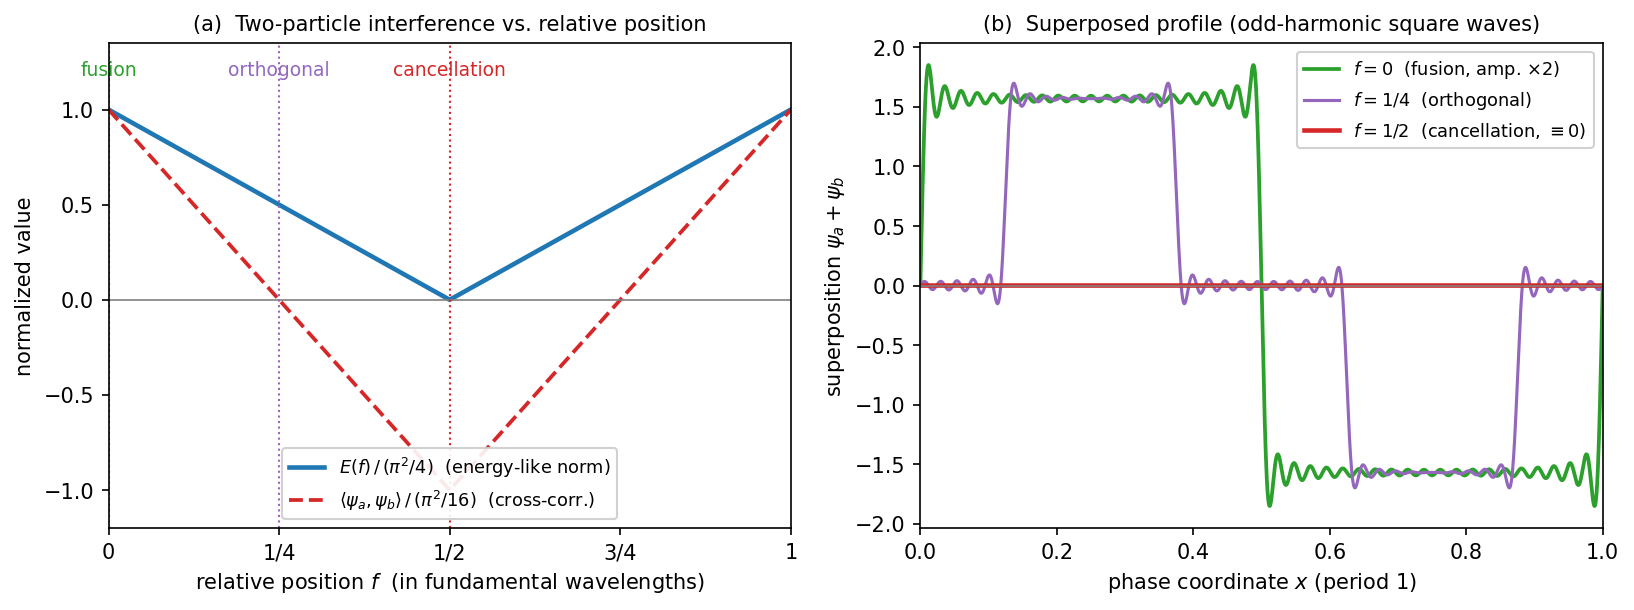
\includegraphics[keepaspectratio,alt={Figure 1}]{p15_interference.png}}
\caption{Figure 1}
\end{figure}

\textbf{Figure 1}: (a) For relative position \(f\) (in fundamental
wavelengths): the squared norm \(E(f)\) (triangle wave, blue) and the
cross-correlation \(\langle\psi_a,\psi_b\rangle\) (red dashed). Fusion
at \(f=0\), orthogonality (zero cross-correlation) at \(f=1/4\),
complete cancellation (\(E=0\)) at \(f=1/2\). (b) The superposed profile
\(\psi_a+\psi_b\) (finite-term odd-harmonic square waves): doubled
amplitude at \(f=0\), orthogonal at \(f=1/4\), identically zero at
\(f=1/2\). The ringing in the waveforms is the Gibbs oscillation from
finite-term truncation.

\begin{center}\rule{0.5\linewidth}{0.5pt}\end{center}

\subsection{§5 Feature points of the relative configuration---fusion,
orthogonality, complete
cancellation}\label{feature-points-of-the-relative-configurationfusion-orthogonality-complete-cancellation}

The cross-correlation
\(\langle\psi_a,\psi_b\rangle=\dfrac{\pi^2}{16}(1-4f)\) expresses the
relation of the two particles concisely. It is a linear function of the
continuous variable \(f\); \(f\) itself is not restricted to discrete
values. Within it, however, three characteristic configurations (feature
points) appear.

\begin{itemize}
\tightlist
\item
  \textbf{\(f=0\) (fusion)}: \(\langle\psi_a,\psi_b\rangle\) maximal.
  The superposition becomes a single square wave of doubled amplitude,
  and the two particles become indistinguishable (effectively appearing
  as one).
\item
  \textbf{\(f=\tfrac14\) (orthogonality)}:
  \(\langle\psi_a,\psi_b\rangle=0\). The two square waves are orthogonal
  and the interference cross-term vanishes. This is a configuration in
  which they \textbf{can coexist independently}, the natural placement
  of two distinguishable particles.
\item
  \textbf{\(f=\tfrac12\) (complete cancellation)}:
  \(\langle\psi_a,\psi_b\rangle\) minimal (\(-\pi^2/16\)). Since
  \(\psi_b=-\psi_a\) (a square wave shifted by half a period reverses
  sign), \(\psi\equiv0\). In this superposition convention the composite
  field vanishes and no non-trivial two-particle mode remains.
\end{itemize}

Therefore, within the continuous relative position \(f\), there appear
\textbf{discrete feature points} corresponding to fusion, orthogonality,
and complete cancellation. In particular, the orthogonal
configurations---where the interference cross-term vanishes and the two
can coexist independently---form a discrete sequence at
\(f=\tfrac14,\tfrac34,\tfrac54,\dots\) (odd \(\times\tfrac14\)), with
spacing (pitch) of half a wavelength. The orthogonal configurations sit
exactly midway between the fusion points (integer \(f\)) and the
complete-cancellation points (half-integer \(f\)).

To say that ``the relative position is discretized,'' one would have to
impose a separate selection principle, e.g.~restricting the admissible
configurations to the orthogonal ones (independent coexistence). This
note does not impose that; it keeps \(f\) a continuous variable and
merely observes that the discrete sequence of orthogonal configurations
appears as feature points within it. The spacing of this orthogonal
sequence (half a wavelength) is not due to an external lattice, but is
\textbf{the scale given by the particle's own spread (fundamental
wavelength \(\propto1/\nu_{R,a}\), preceding note {[}1{]})}. The smaller
the spread (the larger \(\nu_{R,a}\)), the finer the spacing of the
orthogonal sequence.

Furthermore, of these three feature points, the \textbf{existence} of
fusion (\(f=0\)), orthogonality (\(f=\tfrac14\)), and complete
cancellation (\(f=\tfrac12\)) is \textbf{not specific to the square wave
but universal to any profile with half-wave antisymmetry (odd harmonics
only)}. Indeed, for a general odd-harmonic profile
\(\sum_{n\ \mathrm{odd}}a_n\sin(2\pi n(x-x_a))\) the cross-correlation
is \(\tfrac12\sum_{n\ \mathrm{odd}}a_n^2\cos(2\pi n f)\), and at
\(f=\tfrac14\) we have \(\cos(n\pi/2)=0\) for every odd \(n\), so they
are orthogonal independently of the amplitudes \(a_n\). The complete
cancellation at \(f=\tfrac12\) likewise follows immediately from
half-wave sign reversal. Moreover, the modulation factor
\(\cos(n\pi f)\) on each harmonic (point 2 of §3) is a geometric factor
arising from the offset of the two copies, independent of the amplitudes
\(a_n\); hence the comb modulation---which harmonic vanishes where, and
that higher harmonics are filtered out faster in \(f\)---is also
\textbf{universal}. By contrast, only the fact that the envelope
\(\sum_{n\ \mathrm{odd}}a_n^2\cos^2(n\pi f)\) formed by squaring and
summing this modulation becomes \textbf{exactly piecewise linear (a
triangle wave)} is specific to the square-wave (Walsh-like) choice with
amplitudes \(1/n\) (a pure sine gives \(E\propto\cos^2(\pi f)\), which
is not linear). Thus the three feature points and the comb
modulation---the central message of this note---are \textbf{robust,
detached from the arbitrariness of the waveform choice}, and only the
linear (triangle-wave) envelope of \(E(f)\) is a consequence of the
square-wave choice.

This behavior \textbf{corresponds structurally} to the known structure
whereby discrete levels arise from the self-consistency condition of a
standing wave (quantization of states by standing waves). This note
merely observes the correspondence and claims no derivation of
quantization.

\begin{center}\rule{0.5\linewidth}{0.5pt}\end{center}

\subsection{§6 Admissibility of overlap and a structural correspondence
with quantum
statistics}\label{admissibility-of-overlap-and-a-structural-correspondence-with-quantum-statistics}

In the previous section we simply superposed the two particles as a sum
\(\psi_a+\psi_b\). When superposing identical particle-like states,
there are two ways: the sum (symmetrization) or the difference
(antisymmetrization). The admissibility of \textbf{complete overlap}
(\(f=0\)) is reversed between the two.

\textbf{Symmetric combination}
\(\psi_{+}=\psi_a+\psi_b=\displaystyle\sum_{n\ \mathrm{odd}}\frac{2}{n}\cos(n\pi f)\,\sin(2\pi n(x-x_c))\)

\begin{itemize}
\tightlist
\item
  \(f=0\): \(2\psi_a\) (maximal constructive interference, doubled
  amplitude). At complete overlap a \textbf{non-trivial composite mode
  remains}. This corresponds to the behavior of stacking into the same
  mode.
\item
  \(f=\tfrac12\): the composite field vanishes.
\end{itemize}

\textbf{Antisymmetric combination}
\(\psi_{-}=\psi_a-\psi_b=\displaystyle\sum_{n\ \mathrm{odd}}\frac{2}{n}\sin(n\pi f)\,\cos(2\pi n(x-x_c))\)

\begin{itemize}
\tightlist
\item
  \(f=0\): since \(\sin(0)=0\), \(\psi_{-}\equiv0\). \textbf{At complete
  overlap the composite field vanishes, and the antisymmetric
  combination cannot represent a non-trivial two-particle mode.}
\item
  \(f=\tfrac12\): maximal, since \(\sin(n\pi/2)=\pm1\).
\end{itemize}

That is, the amplitude-modulation factor is \(\cos(n\pi f)\) for the
symmetric combination and \(\sin(n\pi f)\) for the antisymmetric
combination, so the admissibility at \(f=0\) is exactly exchanged. In
other words,

\[\text{"can they completely overlap?"}\ \Longleftrightarrow\ \text{"symmetric or antisymmetric combination?"}\]

The symmetric combination, in which complete overlap is admissible,
shows the behavior of stacking into the same state (boson-like); the
antisymmetric combination, which vanishes upon complete overlap, shows a
behavior corresponding to the exclusion of the same configuration
(Pauli-like).

This branching of overlap-admissibility by symmetrization /
antisymmetrization \textbf{corresponds structurally} to the exchange
symmetry of bosons / fermions in quantum statistics.

However, the \(\psi_\pm=\psi_a\pm\psi_b\) treated here is a
\textbf{one-body superposition} of two profiles on a single relational
coordinate \(x\), not the symmetrization / antisymmetrization on the
two-body configuration space \((x_1,x_2)\),
\(\Psi_\pm(x_1,x_2)=\psi_a(x_1)\psi_b(x_2)\pm\psi_a(x_2)\psi_b(x_1)\)
(symmetric \(\Psi_+\) being bosonic, antisymmetric \(\Psi_-\)
fermionic). The two are different objects. Indeed, at the coincidence
point \(f=0\) where statistics genuinely act, the vanishing of the
antisymmetric combination reduces to the waveform-independent algebraic
identity \(g-g=0\). Hence the ``structural correspondence'' with quantum
statistics in this note is a correspondence in the \textbf{limited sense
of an isomorphism of the algebraic vanishing (\(A-A=0\)) at the
coincidence point}, not a derivation of two-body exchange symmetry.

Also, the fact that the antisymmetric combination carries a sign
reversal under exchange shares a \textbf{formal commonality of sign
reversal} with a mode that reverses sign upon one full turn around the
closed phase (the half-integer / double-cover type). However, that the
property of the permutation group \(S_2\) and the topological property
of the rotation group are non-trivially connected is itself the deep
content of the spin-statistics theorem; this note does not assert that
connection and confines itself to pointing out the formal commonality.

From the above, the correspondence in this note is merely an observation
at the level of the superposition convention (symmetrization /
antisymmetrization), and is not an explanation of the spin-statistics
theorem itself, which links the symmetry of the wavefunction with spin.
This note merely observes the correspondence and claims no derivation of
quantum statistics.

\begin{center}\rule{0.5\linewidth}{0.5pt}\end{center}

\subsection{§7 The case of unequal frequencies
(observation)}\label{the-case-of-unequal-frequencies-observation}

So far we have treated the case where the two particles have equal
frequency. We state the case of unequal frequencies briefly, as an
observation.

Here we restrict to the case where the two frequencies are represented
as \textbf{integer modes} on a common period line (or where a common
period can be taken for a rational ratio). Sines of integer modes are
orthogonal over the closed interval
(\(\int_0^1\sin(2\pi m x)\sin(2\pi n x)\,dx=0\), \(m\neq n\) integers).
Hence the cross-correlation of the two particles arises \textbf{only
from shared harmonics}:

\[\langle\psi_a,\psi_b\rangle=\sum_{\omega\,\in\,\text{shared}}\frac{1}{2\,m_\omega\,l_\omega}\cos(2\pi\omega f),\qquad \omega=m\,\nu_a=l\,\nu_b\ (m,l\ \text{odd}).\]

If no harmonic is shared, \(\langle\psi_a,\psi_b\rangle=0\) and
interference vanishes regardless of the relative position \(f\). Then
the two particles can coexist independently at any relative position,
and the \textbf{placement is free}.

Whether sharing occurs is determined by the integer structure of the
frequency ratio. Writing \(\nu_a/\nu_b\) as an irreducible fraction
\(r/s\), the odd-harmonic ladders \(\nu_a\{1,3,5,\dots\}\) and
\(\nu_b\{1,3,5,\dots\}\) share a point exactly when \textbf{\(r\) and
\(s\) are both odd} (then there exist odd \(m,l\) with \(m s=l r\)).
Normalizing to integer frequencies as
\(\nu_a=2^{\alpha}p',\ \nu_b=2^{\beta}q'\) (\(p',q'\) odd), this
corresponds to \(\alpha=\beta\) (matching of the power-of-2 component).
When \(r\) and \(s\) differ in parity (\(\alpha\neq\beta\)), no odd
harmonic is shared and the result is complete orthogonality = free
placement.

If \(\nu_a/\nu_b\) is irrational, there is no common period, and the
very setting of this note---``a single closed phase line of period
\(1\)''---does not hold. The statement that interference vanishes in
this case is a heuristic extrapolation outside the present setting, not
a conclusion within the framework of this note.

In summary, the following correspondences are observed in the framework
of this note.

\begin{itemize}
\tightlist
\item
  \textbf{Equal frequency (identical particles)}: all harmonics
  coincide, and the strong interference, sharp feature points, and
  statistical behavior of §3--§6 appear.
\item
  \textbf{Unequal but commensurate (odd ratio)}: only higher harmonics
  are shared (with small weight \(1/(m l)\)), and weak interference and
  weak feature points remain.
\item
  \textbf{Incommensurate (different power of 2)}: interference vanishes,
  free placement, independence (an irrational ratio has no common period
  and lies outside the present setting).
\end{itemize}

This \textbf{corresponds structurally} to the known fact that exchange
statistics act only on identical particles and not on distinguishable
ones. This note merely observes the correspondence.

\begin{center}\rule{0.5\linewidth}{0.5pt}\end{center}

\subsection{§8 What this note does not
treat}\label{what-this-note-does-not-treat}

This note does not treat the following:

\begin{itemize}
\tightlist
\item
  the coordinate-invariant formulation of the relative configuration /
  interference on a general \(S^4(R_{\mathrm U})\) (this note is
  restricted to the one-dimensional minimal setting);
\item
  derivation of the spin-statistics theorem, the Hilbert-space
  structure, or quantum field theory;
\item
  judgment of the stability or dynamics of a local mode (equations of
  motion, energy functional);
\item
  fluctuations of particle number / uncertainty of existence, or
  correspondence with virtual particles;
\item
  interference of three or more particles, the higher-dimensional
  structure of the configuration space;
\item
  identification of the interference structure of this note with
  concrete quantum numbers, spectra, or actual statistics.
\end{itemize}

These are extension topics that could be examined if the observation of
two-particle interference of this note were further developed. At the
present stage, however, they go beyond the scope of this note.

\begin{center}\rule{0.5\linewidth}{0.5pt}\end{center}

\subsection{§9 Scope of the claims of this
note}\label{scope-of-the-claims-of-this-note}

The claims of this note are limited to the following range.

First, on a closed one-dimensional relational setting, the spectrum of
the superposition of two equal-frequency rectangular standing waves
stays on the same odd-harmonic ladder, with each harmonic amplitude
given by \(A_n=\tfrac{2}{n}\cos(n\pi f)\).

Second, its total squared norm (energy-like quantity) is the triangle
wave \(E(f)=\tfrac{\pi^2}{4}(1-2f)\) (\(0\le f\le\tfrac12\)), equal to
the autocorrelation of a square wave.

Third, within the continuous relative position \(f\) there appear
discrete feature points: fusion at \(f=0\), orthogonality (independent
coexistence) at \(f=\tfrac14\), and complete cancellation (the composite
field vanishes, no non-trivial mode remains) at \(f=\tfrac12\).

Fourth, depending on whether the superposition is symmetrized or
antisymmetrized, complete overlap is admissible (boson-like) or makes
the composite field vanish, i.e.~exclusive (fermion-like).

Fifth, for unequal frequencies, interference arises only from shared odd
harmonics, and without sharing it vanishes, giving free placement.
Whether sharing occurs is determined by whether \(\nu_a/\nu_b\) is an
odd ratio (matching of the power-of-2 component).

Sixth, all of the above are \textbf{observations of structural
correspondence} with known structures (standing-wave quantization, the
exchange symmetry of quantum statistics), not derivations of them.

\begin{center}\rule{0.5\linewidth}{0.5pt}\end{center}

\subsection{Summary}\label{summary}

The central observation of this note can be summarized as follows.

\begin{quote}
When two particle-like states with a spread phase are superposed as
rectangular standing waves on a closed one-dimensional relational
setting, discrete feature points (fusion, orthogonality, complete
cancellation) appear within the continuous relative position, and the
admissibility of complete overlap (boson-like / fermion-like) is divided
according to symmetrization / antisymmetrization. These appear as closed
elementary Fourier-series computations.
\end{quote}

Whereas the preceding note {[}1{]} fixed the geometric stage and the
spread of a single particle, this note presents, as an observation, the
relational structure that appears when two particles are placed on that
stage---the feature points of the relative configuration and a
structural correspondence with quantum statistics. The computation
itself is complete as a Fourier analysis of square waves on a period-1
closed phase line; the central projection and subjective geometry
\(S^4(R_{\mathrm U})\) of §1 are its motivating framework. The
coordinate-invariant formulation on a general \(S^4(R_{\mathrm U})\),
three or more particles, and dynamics and stability are made the subject
of subsequent notes.

\begin{center}\rule{0.5\linewidth}{0.5pt}\end{center}

\subsection{References}\label{references}

{[}1{]} N. Kihara (2026). \emph{Central projection of a vacuum universe
and particle-like states with a spread phase}. Observational note (same
author; preceding note). Concept DOI:
\href{https://doi.org/10.5281/zenodo.20543044}{10.5281/zenodo.20543044}.

{[}2{]} N. Kihara (2026). \emph{A thought experiment on a model particle
(continued)---the fifth frequency and composite curvature seen from the
sum-to-zero condition}. Observational note (same author). Concept DOI:
\href{https://doi.org/10.5281/zenodo.20535894}{10.5281/zenodo.20535894}.

{[}3{]} N. Kihara (2026). \emph{Definition of the spherical projection
\(\sigma_R\) (radial projection)---the foundational map of the
central-projection series}. Observational note (same author). Concept
DOI:
\href{https://doi.org/10.5281/zenodo.20462569}{10.5281/zenodo.20462569}.

{[}4{]} T. W. Körner (1988). \emph{Fourier Analysis}. Cambridge
University Press. (Fourier series of a square wave, Parseval's relation,
autocorrelation and the triangle wave)

(Note: external references use the Concept DOI.)

\begin{center}\rule{0.5\linewidth}{0.5pt}\end{center}

\subsection{Revision history}\label{revision-history}

\begin{itemize}
\tightlist
\item
  \textbf{v1.0 (2026-06)}: Initial version (publication candidate).
  Treats the minimal case (two equal-frequency particles, closed
  one-dimensional setting) of the multi-particle interference that the
  preceding note {[}1{]} deferred. Presents, all as observations of
  structural correspondence: the spectrum of the same-harmonic
  superposition \(A_n=\tfrac{2}{n}\cos(n\pi f)\); the triangle-wave
  squared norm \(E(f)=\tfrac{\pi^2}{4}(1-2f)\) (the autocorrelation of a
  square wave); the discrete feature points appearing within the
  continuous relative position (fusion \(f{=}0\), orthogonality
  \(f{=}\tfrac14\), complete cancellation \(f{=}\tfrac12\)); the
  reversal of overlap-admissibility by symmetrization /
  antisymmetrization (boson-like / fermion-like); and, for unequal
  frequencies, that the presence of shared odd harmonics (irreducible
  ratio \(r/s\) with both odd = matching power-of-2 component) governs
  interference. Incorporating external review (ChatGPT, Grok, Gemini,
  Claude.ai): terms weakened from ``discretization'' to ``appearance of
  discrete feature points,'' from ``forbidden'' to ``complete
  cancellation / no non-trivial mode remains,'' and from ``emergence of
  statistics'' to ``structural correspondence with quantum statistics'';
  \(E(f)\) stated as an energy-like quantity based on the Parseval
  squared norm, not physical energy; the square wave stated as a global
  standing profile on the relational-phase coordinate (not a localized
  wave packet); §7 made rigorous by restricting to integer modes /
  rational ratios; §2 minimally notes the functional reason for the
  square-wave choice (no physical meaning to wave height; shape
  deferred); §6 clarifies that \(\psi_\pm\) is a one-body superposition,
  not the two-body antisymmetrization, the correspondence being a
  limited isomorphism of the algebraic vanishing \(A-A=0\) at
  coincidence, and weakens the double-cover relation to a ``formal
  commonality of sign reversal''; §5 separates universal
  vs.~waveform-specific (feature points and comb modulation universal;
  only the triangle-wave linear envelope specific to the \(1/n\)
  choice). Figure 1 added in §4. No derivation of the spin-statistics
  theorem or quantum statistics is claimed; the general \(S^4\)
  formulation, dynamics, and three or more particles are deferred to
  subsequent notes.
\end{itemize}

\end{document}
